\documentclass[10pt]{article}
\usepackage[margin=2cm]{geometry}
\usepackage{amsmath,amssymb}
\usepackage{tikz}
\usetikzlibrary{arrows.meta,positioning,calc}
\usepackage[hidelinks]{hyperref}
\title{Closing walks: the signed paths a vertex pair would close}
\author{hymeko/graph, plan 2026-10-10 (CORE.YAML item \texttt{hymeko\_graph}: justification and migration)}
\date{Created-at: 2026-10-10 13:03 CEST.\quad ETA: about 1.5\,h (function, tests, gate).}
\begin{document}
\maketitle

\paragraph{Approval.} The user, 2026-10-10 13:0x: ``megadva a lehet\H{o}s\'eg hogy jav\'its a hymeko\_graphot egy
\'uj feature branchel''. Branch \texttt{feat/closing-walks} from \texttt{88f4847} (\texttt{hymeko\_core}
\texttt{219d4f4}, the revision Nagare pins), so Nagare can take it without a core bump.

\section*{Justification}
Nagare's signed-link models pool, for a query edge $(u,v)$, the cycles that contain it. Enumerated over every edge,
those cycles' signs carry the query's own sign: the label leaks. Enumerated over the training edges, no cycle
contains a held-out edge, and the models have no context at all (Nagare plan 2026-10-10-framework-reproductions,
Amendments 5 and 7, measured).

The leak-free form of the same evidence is the set of paths $u\to w_1\to\dots\to v$ of length $L\ge2$ over the visible
edges, never through the pair itself: the cycles the pair would close, without its sign. $L=2$ is the triangles
(common neighbours), $L=3$ the 4-cycles. Paths between a given pair are a generic signed-graph algorithm, and this
crate is their one owner (CORE.YAML: ``cycle and walk enumeration''). Nagare must not grow a second enumerator.

\section*{Interface (additive)}
\begin{itemize}
\item \texttt{ClosingWalkRequest \{ per\_pair\_cap: Option<usize>, seed: u64, resolution:
  MultiEdgeSignResolution \}}.
\item \texttt{enumerate\_closing\_walks(graph, visible, pairs, len, request) -> ClosingWalks}.
\item \texttt{ClosingWalks \{ len, vertices, member\_signs, pair\_offsets, dropped, request \}}: tuples grouped
  by pair in the order given. The tuples of pair $p$ are \texttt{pair\_offsets[p]..pair\_offsets[p+1]}; each runs
  from $u$ to $v$ with \texttt{len} edges and carries the \texttt{Walk \{ len \}} family's member signs.
\end{itemize}

\paragraph{Contracts.}
\begin{itemize}
\item \textbf{Graph:} only \texttt{visible} edges are traversed, undirected.
\item \textbf{Walk shape:} simple, with intermediate vertices distinct and outside $\{u,v\}$, and $L\ge2$. A walk
  therefore never traverses the pair.
\item \textbf{Cap:} above it, a pair keeps a uniform reservoir sample seeded by \texttt{(seed, pair index)}.
\item \textbf{Determinism:} the result is byte-identical for equal inputs, whatever the thread count, because each
  pair's sample is independent and the output keeps pair order.
\item \textbf{Signs:} edge signs come from the request's resolution, as \texttt{enumerate\_signed\_tuples} resolves
  them; a walk with an unresolvable edge is dropped and counted.
\end{itemize}

\section*{Migration}
Additive: no existing function, type or result changes, and the existing tests and fingerprints hold. Nagare
consumes it by revision. Merging to \texttt{main} follows Nagare's next \texttt{hymeko\_core} bump, rebased onto
\texttt{origin/main} (core \texttt{b1bc1eb}).

\section*{Tests}
\begin{itemize}
\item On fixtures, against a brute-force reference: the walks equal every simple path of length $L$ between the pair
  over the visible edges, for $L=2,3$.
\item No walk traverses the pair or an invisible edge.
\item The member signs follow the \texttt{Walk} rule under each resolution.
\item A capped pair keeps the cap, a reproducible sample, and the same bytes at 1 and 4 threads.
\item Refusals: $L<2$, a pair with $u=v$, a vertex out of range.
\end{itemize}
\paragraph{Performance.} Per pair the work is the paths explored: $\deg(u)$ for $L=2$, $\sum_{w\in N(u)}\deg(w)$ for
$L=3$. It is measured on Bitcoin-Alpha (24\,186 queries) through Nagare before any campaign.
\paragraph{Rollback.} Delete the branch; nothing on \texttt{main} changes.

\begin{center}
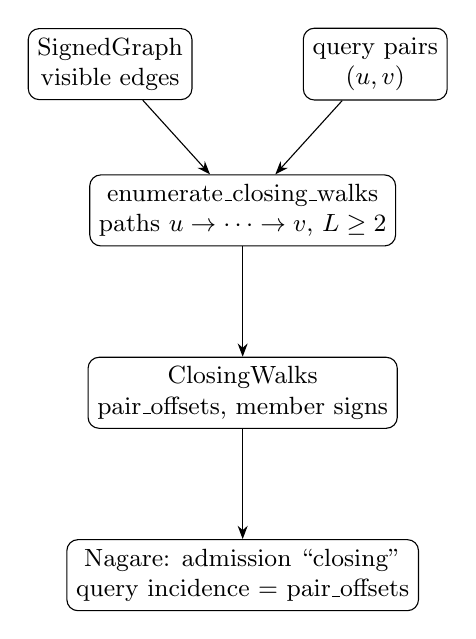
\begin{tikzpicture}[node distance=1.4cm, every node/.style={draw, rounded corners, font=\small, align=center}]
\node (g) {SignedGraph\\visible edges};
\node (p) [right=of g] {query pairs\\$(u,v)$};
\node (e) [below=of $(g)!0.5!(p)$] {enumerate\_closing\_walks\\paths $u\to\dots\to v$, $L\ge2$};
\node (r) [below=of e] {ClosingWalks\\pair\_offsets, member signs};
\node (n) [below=of r] {Nagare: admission ``closing''\\query incidence = pair\_offsets};
\draw[-Stealth] (g) -- (e); \draw[-Stealth] (p) -- (e); \draw[-Stealth] (e) -- (r); \draw[-Stealth] (r) -- (n);
\end{tikzpicture}
\end{center}

\end{document}
